%!TEX root = ../dissertation.tex

\Chapter{Supplementary information for Chapter~\ref{sec:memory}}

\section{Deviations from pre-registration}\label{app:deviation}

After pre-registering and running the experiments, we discovered a flaw in the implementation of the lesioned models without meta-level control. In our first implementation, stopping times and fixation durations were sampled directly from the empirical distribution in the human data (discretized into 100ms time steps). We reasoned that this would give the model the best chance of capturing the human behavior without a metacognitive component. However, we later realized that this approach effectively prevents the model from utilizing non-decision time, as any non-decision time would be added to a distribution that already perfectly matches the human data.

After realizing this, we implemented the more flexible lesioned model with stopping times and fixation durations drawn from arbitrary Gamma distributions, as reported in the main text. Note that this model has more free parameters in the two-item case, thus we also decided to fit the lesioned model to data in Experiment 2 (contrary to our intention to use the fitted parameters from Experiment 1). The predictions of the original model for both experiments are shown in Figures~\ref{fig:exp1_rt_alt}-\ref{fig:commitment_alt}.

This analysis also revealed that two of the effects which we had believed to be evidence of meta-level control could in fact be produced by the model without meta-level control. The first such effect is shown in \figref{fig:exp1_cum}{B}. The original logic of this plot was to look at how strength affects the decision to skip a trial over time, after factoring out the effect of strength on recall (which in turn prevents skipping). With a low or moderate non-decision time distribution, this effect cannot be captured by a model without meta-level control. However, when non-decision time is a sufficiently large portion of total response time, the effect can be produced through mechanistic means. Given this, we could not provide a useful interpretation of the effect, and thus removed it from the main text.

The second effect is the prediction that final fixations are longer than non-final fixations (\figref{fig:commitment}{A}). We elected to keep this effect in the main text because its interpretation as an indication of rational metamemory was further supported by the additional analysis of the distribution of pretest accuracy for long fixations (\figref{fig:commitment}{B}).

\begin{figure*}[]
  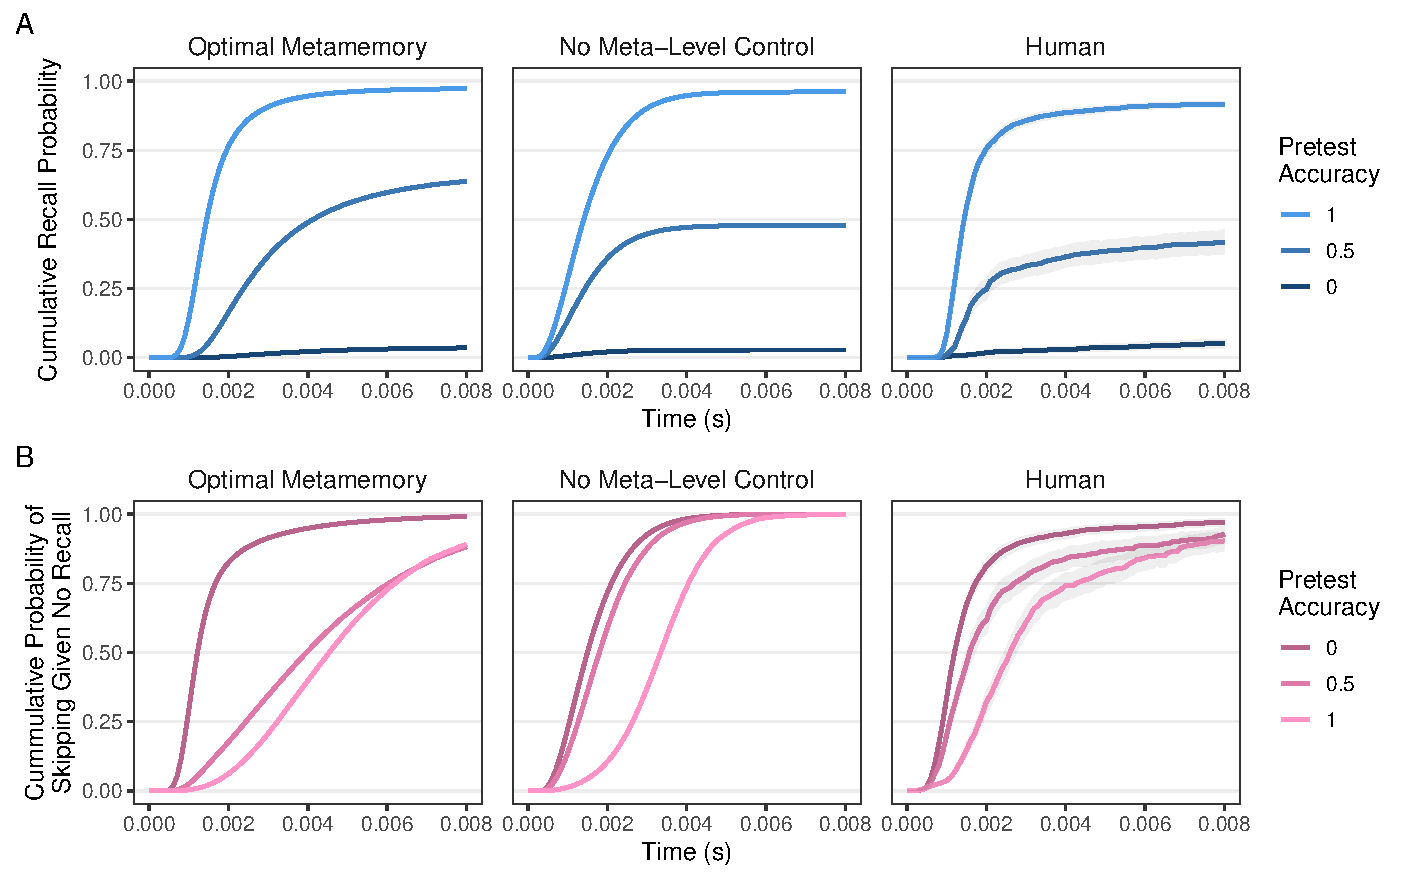
\includegraphics[scale=.75]{figs/memory/exp1/cum_probs.pdf}
  \caption{%
    Timecourse of recall and stopping.
    (A) For each time point (in 100ms steps), the proportion of trials on which the target was recalled before that point, grouping trials by the accuracy rate of the presented cue in the pretest phase.
    (B) For each time point, the proportion of trials that were skipped before that point, conditioning on the fact that the target had not already been recalled.
    \emph{Note}: Lines show means of participants means and ribbons show 95\% bootstrapped confidence intervals over participant means.
  }
  \label{fig:exp1_cum}
\end{figure*}


\begin{figure*}[]
  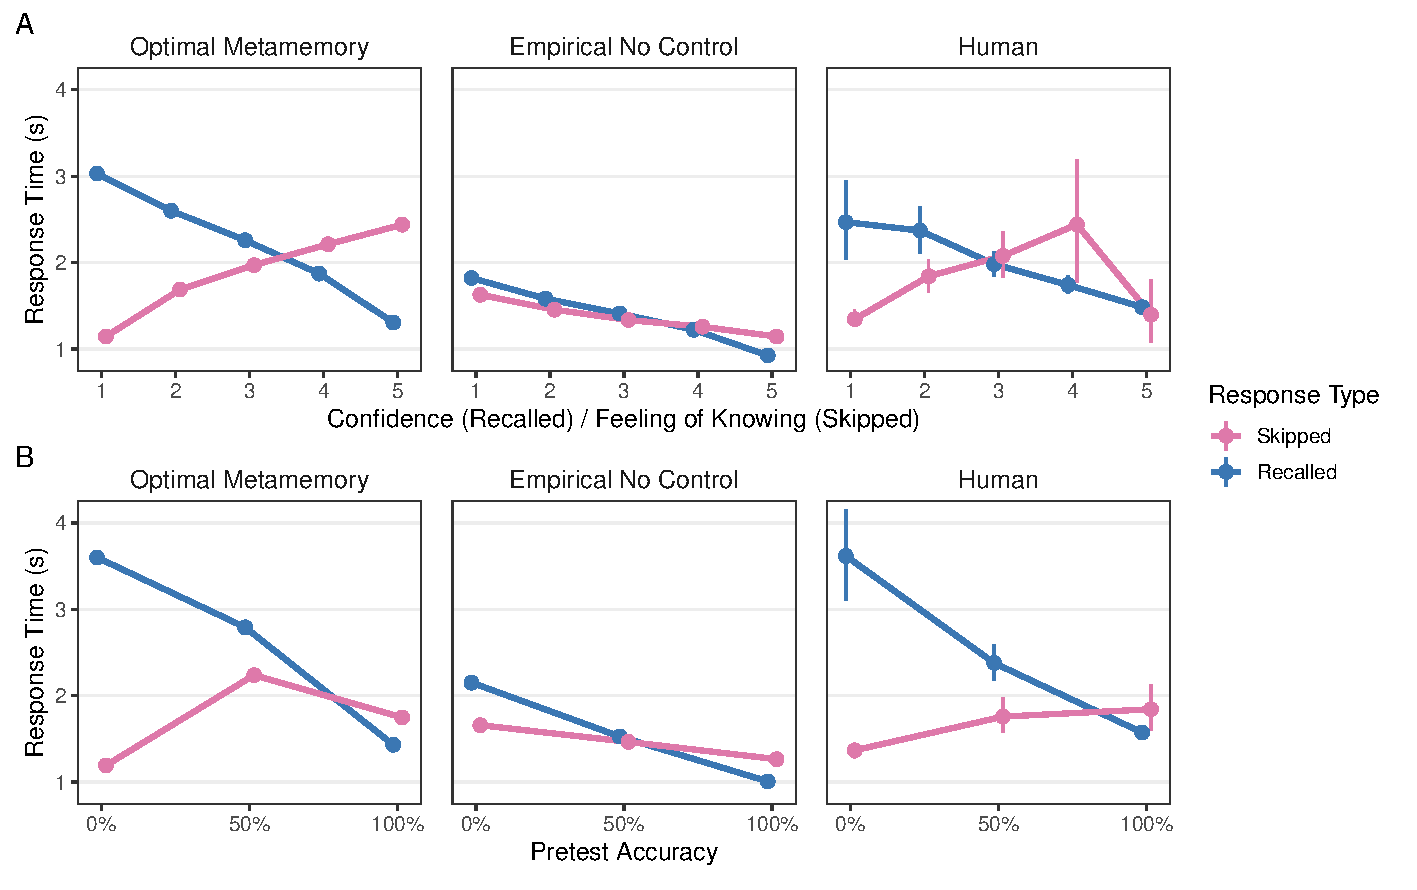
\includegraphics[scale=.75]{figs/memory/exp1_alt/rt.pdf}
  \caption{Alternative version of Figure~\ref{fig:exp1_rt} where the lesioned model draws stopping times from the empirical distribution.}
  \label{fig:exp1_rt_alt}
\end{figure*}

\begin{figure*}[ht]
  \centering
  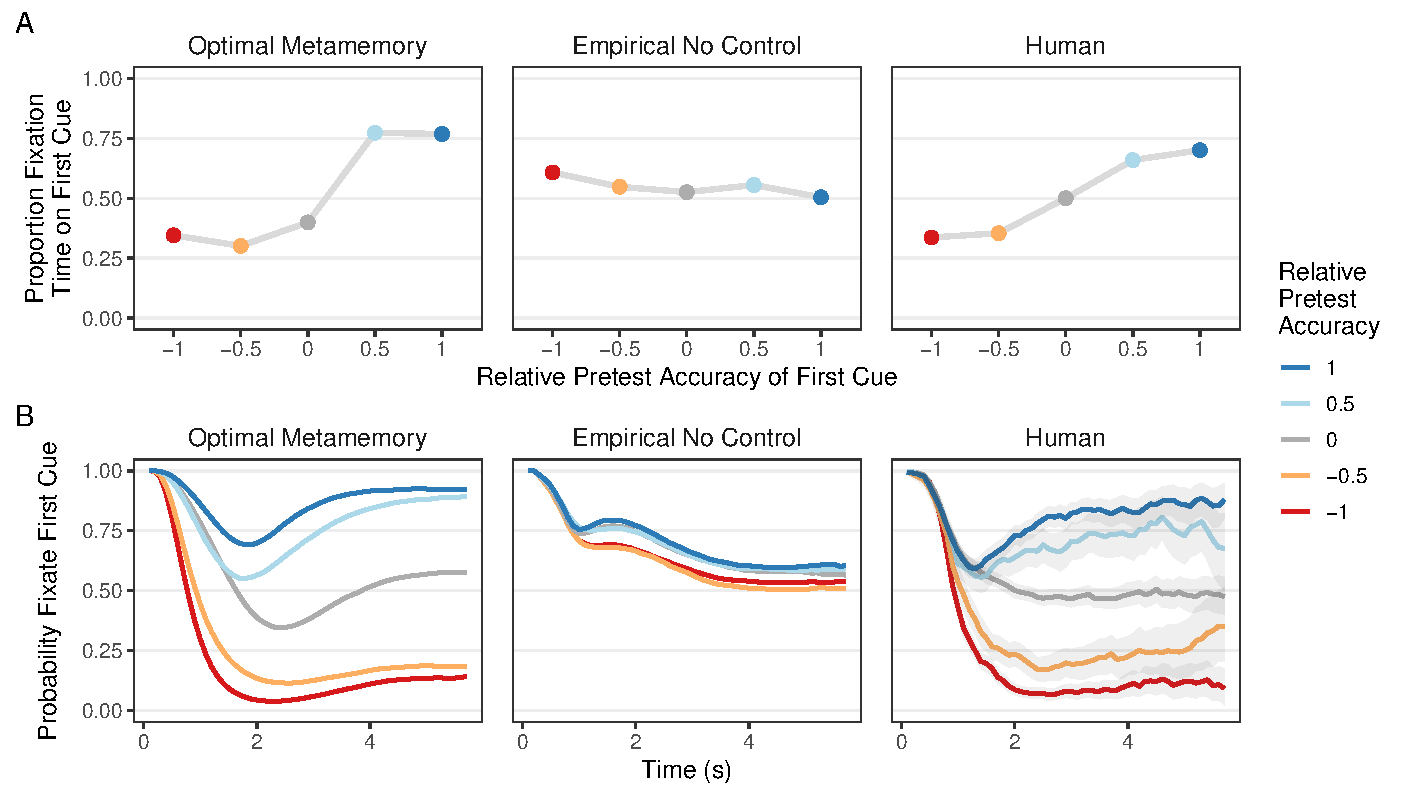
\includegraphics[scale=.75]{figs/memory/exp2_alt/overall_timecourse.pdf}
  \caption{Alternative version of Figure~\ref{fig:timecourse} where the lesioned model draws stopping and switching times from the empirical distribution.}
  \label{fig:timecourse_alt}
\end{figure*}

\begin{figure*}[t]
  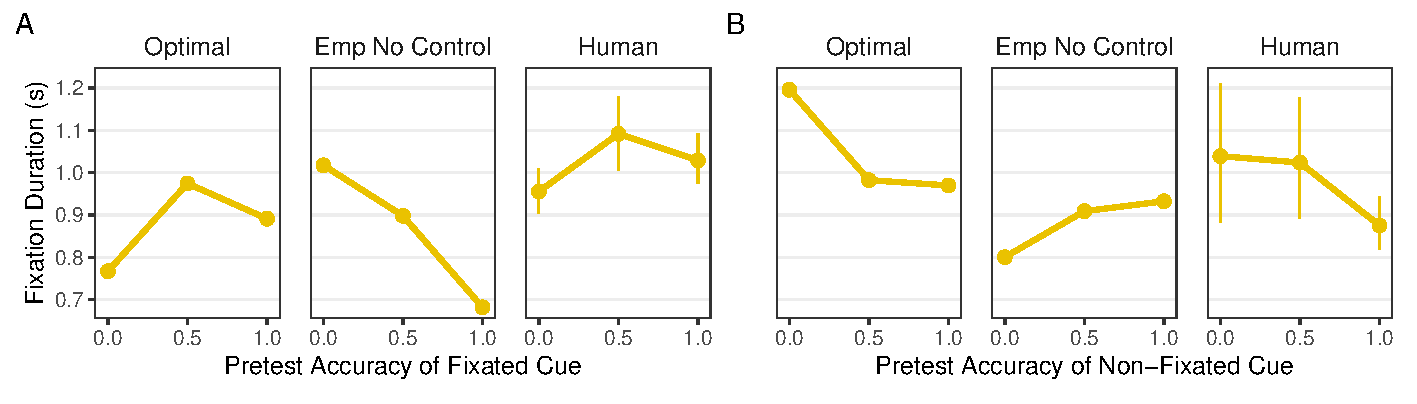
\includegraphics[scale=.75]{figs/memory/exp2_alt/nonfinal.pdf}
  \caption{Alternative version of Figure~\ref{fig:nonfinal} where lesioned model draws stopping and switching times from the empirical distribution.}
  \label{fig:nonfinal_alt}
\end{figure*}

\begin{figure*}[t]
  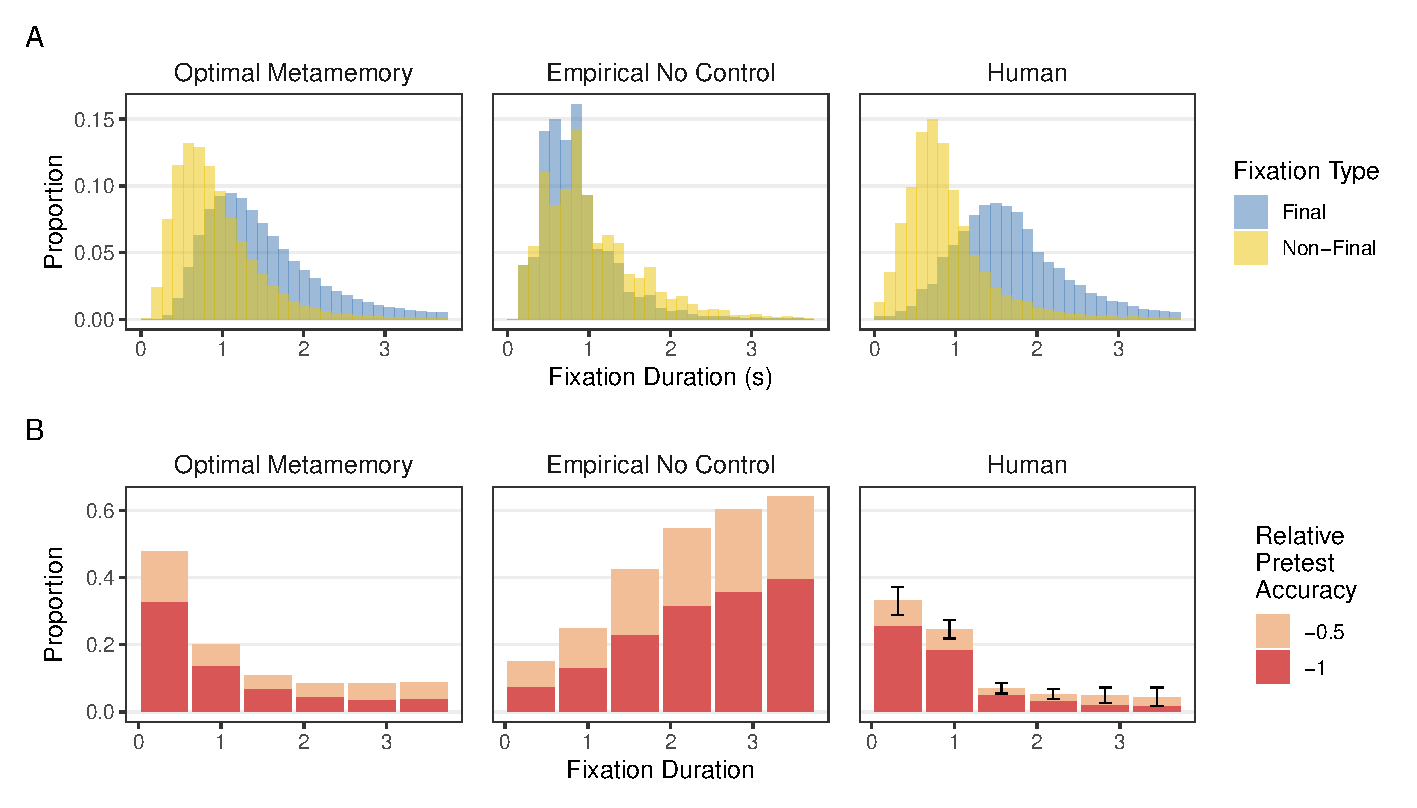
\includegraphics[scale=.75]{figs/memory/exp2_alt/commitment.pdf}
  \caption{Alternative version of Figure~\ref{fig:commitment} where lesioned model draws stopping and switching times from the empirical distribution.}
  \label{fig:commitment_alt}
\end{figure*}


\section{Previously pre-registered experiments}\label{app:previous}

Before running the experiments presented in the main text, we ran another set of large experiments using the exact same experimental design. These were also pre-registered. However, the results from these studies were not conclusive (for different reasons), so we reran them.

For Experiment 1, we initially planned to run 125 participants, and to z-score response times within participants before regressing them on pretest accuracy. This analysis yielded a marginally significant effect of pretest accuracy on response time for skip trials ($p=.062$). The original pre-registration is available at \url{https://aspredicted.org/ss8x3.pdf}. While analyzing the data, we also discovered that the z-scoring step actually reduced statistical power, as it selectively diminished the contribution of participants who showed the effect most robustly (and thus had more variable response times). We thus eliminated the z-scoring step, pre-registered the slightly modifide analysis, and reran the experiment with a target of 500 participants. Note that the mixed effects analysis still accounts for individual variability in both average response times and sensitivity to pretest accuracy.

for Experiment 2 (which was actually run first), we had planned to use a definition of memory strength that combined response time and accuracy on the pretest trials. The logic was that a fast response indicated a stronger memory; thus, highers response time in the pretest should predict less fixation time in the critical trials. However, we then discovered that response time on the pretest was actually \emph{positively} correlated with fixation durations in the critical trials (contrary to our predictions). This may be due to factors other than memory strength, such as perceptual encoding, which would uniformly increase the amount of time spent looking at an item. Additionally, we had planned a different set of analyses, focusing on the duration of individual fixations as a function of relative strength of the two cues, rather than breaking down the effect of the fixated and non-fixated cues, as we do now. The full pre-registration is available at \url{https://aspredicted.org/ss8x3.pdf}.
Given the extent of the changes we wished to make to the analysis, we pre-registered the new analysis plan and reran the experiment.

As shown in the sections below, all of the results reported in the main text are also significant in this previous sample. We reproduce all the figures from the main text in Figures~\ref{fig:old_exp1_rt}-\ref{fig:old_commitment}.

\subsection{Experiment 1}

We recruited 124 participants and excluded 14 (11\%) participants who did not provide a response on more than 90\% of critical trials. This yielded 110 participants in our final analysis.

Participants were faster to correctly recall targets that they reported greater confidence in ($B = -0.203$, 95\% CI [-0.289, -0.117], $t(119.2)=-4.62$, $p < .001$), but slower to skip targets that they reported higher feeling-of-knowing for ($B = 0.474$, 95\% CI [0.302, 0.646], $t(35.4)=5.41$, $p < .001$). People were likewise faster to recall targets that they had previously recalled correctly ($B = -1.160$, 95\% CI [-1.724, -0.597], $t(41.2)=-4.03$, $p < .001$). More importantly, they were also slower to skip such targets ($B = 0.478$, 95\% CI [0.256, 0.700], $t(151.2)=4.22$, $p < .001$).

\begin{figure*}[ht]
  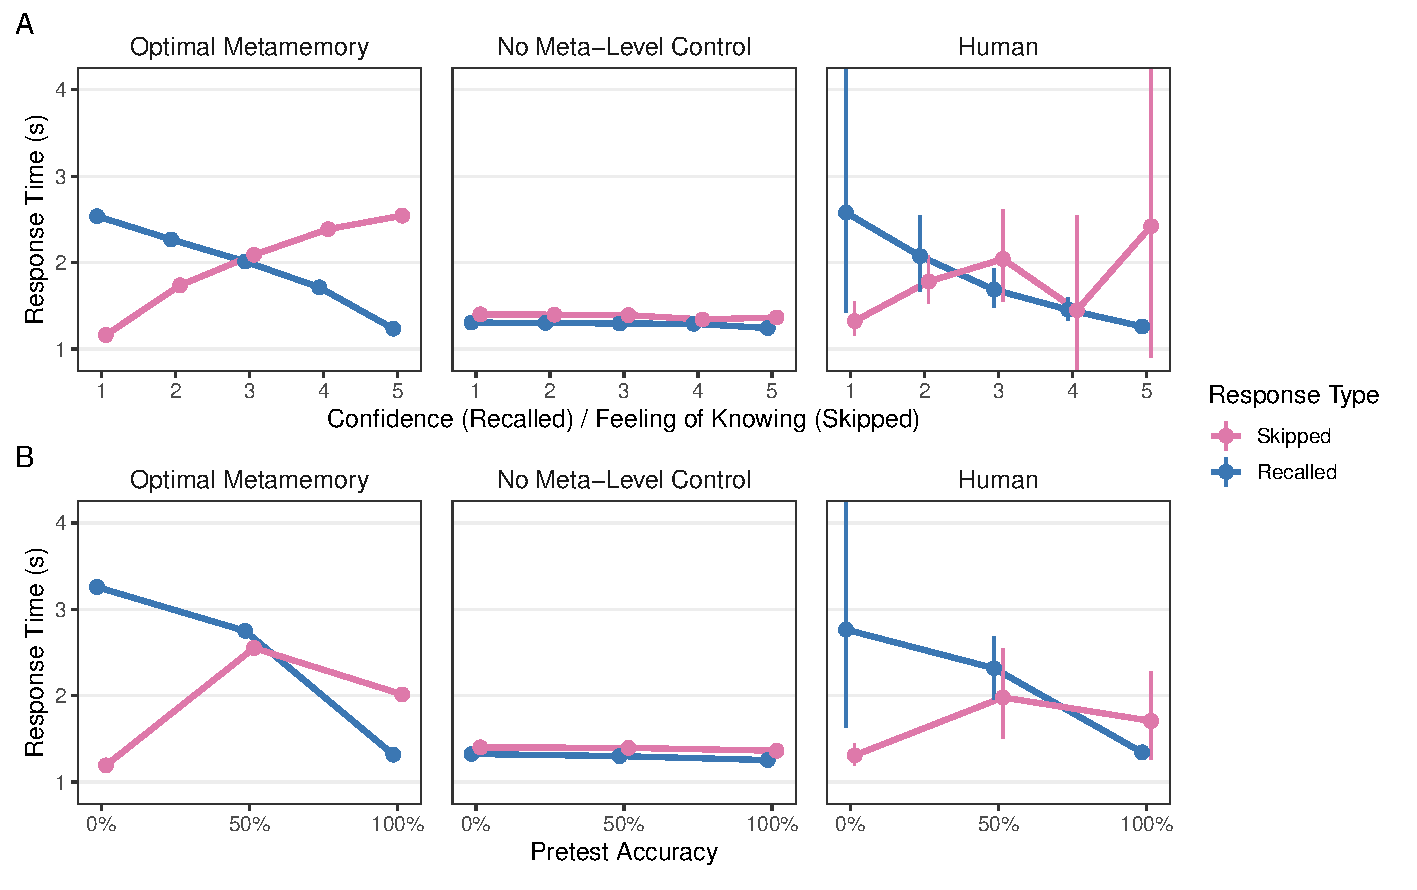
\includegraphics[scale=.75]{figs/memory/old_exp1/rt.pdf}
  \caption{Figure~\ref{fig:exp1_rt} with previous experimental data. The models are fit to the data shown in the plot. We use the same axis limits as in the main text to facilitate comparison (the error bars extend beyond the plotted range).
  }
  \label{fig:old_exp1_rt}
\end{figure*}

\subsection{Experiment 2}

We recruited 459 participants and excluded 65 (14\%) participants who failed to correctly recall a target on more than 50\% of critical trials. This yielded 394 participants in our final analysis.

Participants spent substantially more time looking at cues that were stronger than the other available cue ($B = 0.191$, 95\% CI [0.182, 0.199], $t(572.0)=42.40$, $p < .001$). Their non-final fixations increased with the pretest accuracy of the fixated cue ($B = 0.106$, 95\% CI [0.075, 0.137], $t(230.7)=6.65$, $p < .001$) and decreased with the pretest accuracy of the non-fixated cue ($B = -0.456$, 95\% CI [-0.578, -0.334], $t(59.7)=-7.32$, $p < .001$; first fixations excluded). Final fixations were longer than their non-final fixations ($B = 0.872$, 95\% CI [0.813, 0.930], $t(435.8)=29.29$, $p < .001$). The probability of fixating the weaker memory significantly decreased with fixation duration ($B = -1.482$, 95\% CI [-1.651, -1.313], $z=-17.22$, $p < .001$; logistic regression, excluding trials where the cues had equal pretest accuracy). 

The final result is notable because it confirms the exploratory rational commitment analysis we developed using the new dataset. Thus, although the result in the main text was not pre-registered, the result presented above effectively is; we had finalized the analysis before examining the results it yielded with the old dataset.

\begin{figure*}[ht]
  \centering
  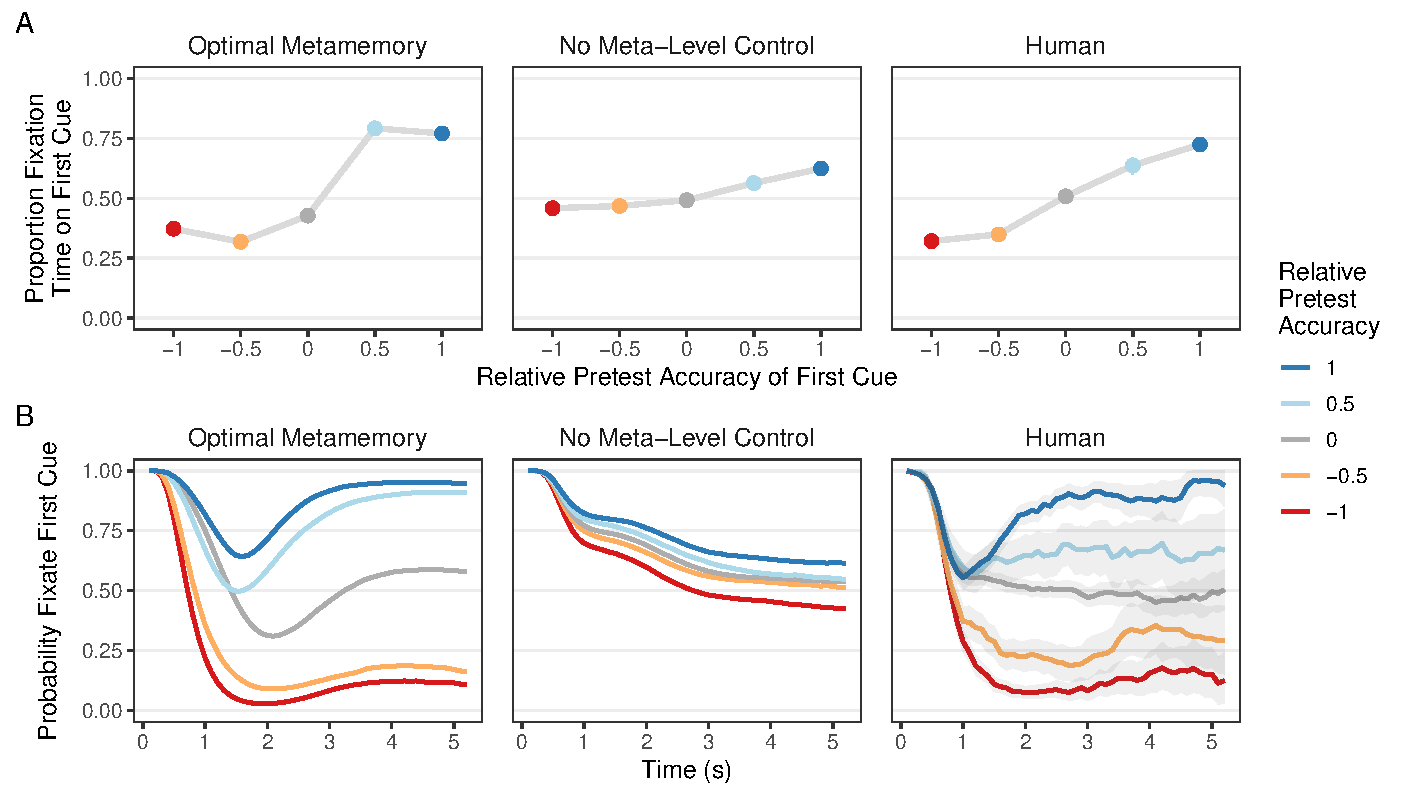
\includegraphics[scale=.75]{figs/memory/old_exp2/overall_timecourse.pdf}
  \caption{Figure~\ref{fig:timecourse} with previous experimental data.
    \label{fig:old_timecourse}
  }
\end{figure*}

\begin{figure*}[t]
  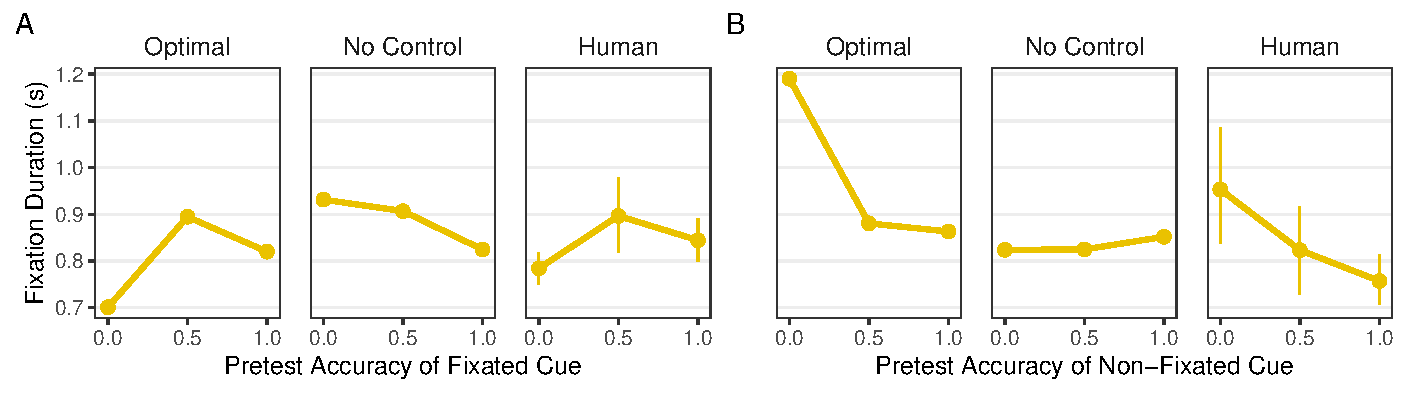
\includegraphics[scale=.75]{figs/memory/old_exp2/nonfinal.pdf}
  \caption{Figure~\ref{fig:nonfinal} with the old previous experimental data.
    \label{fig:old_nonfinal}
}
\end{figure*}

\begin{figure*}[t]
  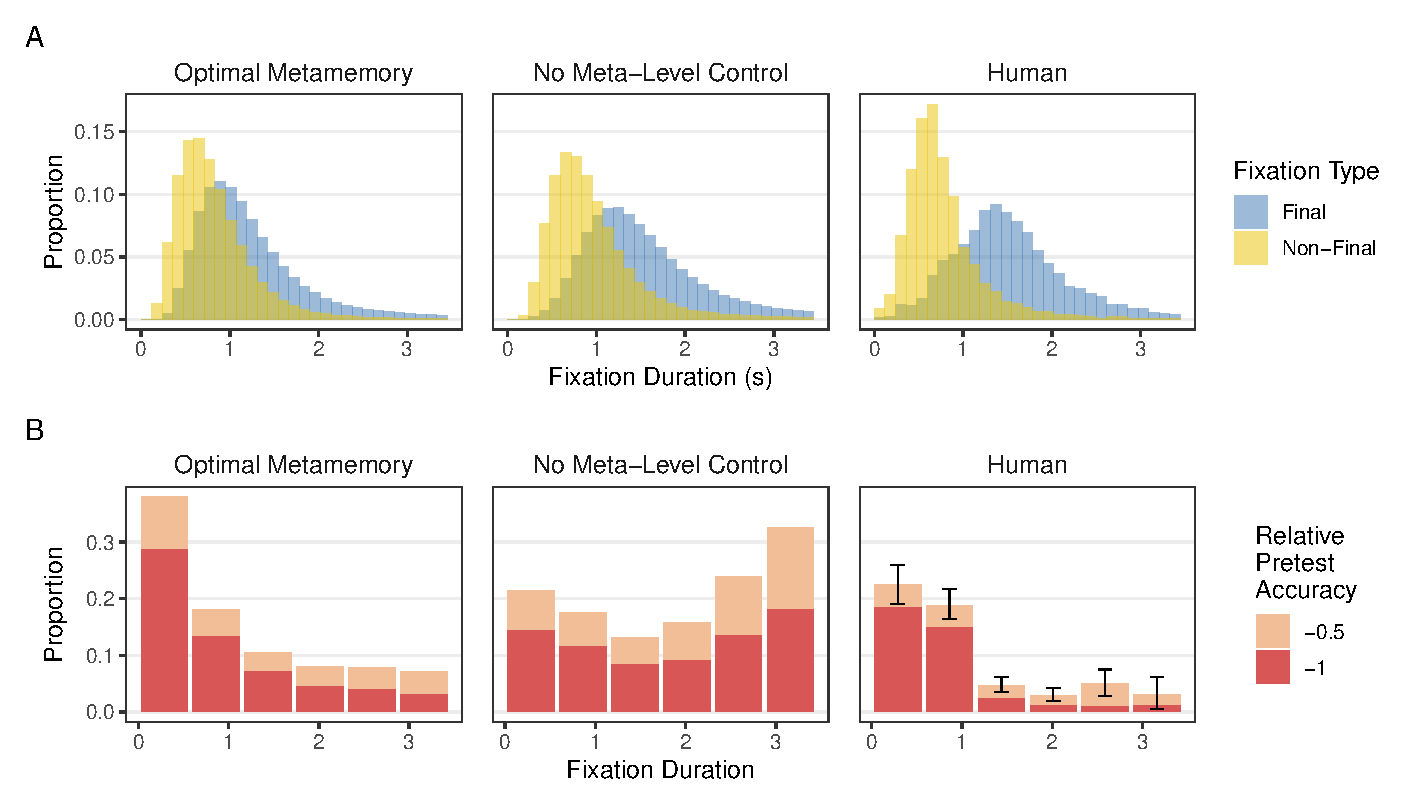
\includegraphics[scale=.75]{figs/memory/old_exp2/commitment.pdf}
  \caption{Figure~\ref{fig:commitment} with previous experimental data.
    \label{fig:old_commitment}
}
\end{figure*}

\section{Optimizing the lesioned model to predict effects}\label{app:lesion-search}

To more conclusively determine which effects are inconsistent with the lesioned model, we conducted a thorough search of the parameter space to see if the model could produce each qualitative effect under any parameter setting. For each experiment, we sampled 100,000 parameter configurations and simulated 100,000 trials for each. From these, we excluded simulations with accuracy below 1\% or above 99\%, as these yield unreliable estimates for effects that condition on accuracy. For similar reasons, in Experiment~2, we excluded configurations for which fewer than 1\% of trials had at least two fixations. For each un-excluded simulation, we then performed a standard linear regression corresponding to the regression we reported in the main text. Next, we selected the 100 configurations who produced the largest effect, as estimated by the lower bound of a 95\% confidence interval (this prevents selecting for models that simply produce highly variable estimates). If the lower confidence bound for any of these was larger than a ``minimal interesting difference'', then we concluded that the lesioned model could produce the effect.

Note that this analysis occurred to us after running the experiment, and was thus not pre-registered.

\subsection{Experiment 1}

As expected, we found that the lesioned model could predict the observed negative effect both judgments ($B = -0.762$; 95\% CI [-0.765, -0.759]) and pretest accuracy ($B = -6.073$; 95\% CI [-6.109, -6.037]) on response time for the correct trials. Note that these are the largest effect sizes we found; they are substantially larger than those seen in the data. Surprisingly, we also found that the lesioned model could predict a substantial positive relationship between judgment and response time on the skip trials ($B = 0.615$; 95\% CI [0.605, 0.626]). However, this model failed to predict the negative relationship on correct trials ($B = 0.052$; 95\% CI [0.050, 0.054]; note that $B$ should be negative). No parameter configuration was able to predict the crossover pattern, with a negative relationship between judgment and response time on correct trials but a positive relationship on skip trials. Furthermore, no configuration was able to predict the positive relationship between pretest accuracy and response time on skip trials (even allowing the relationship for correct trials to be positive).

\subsection{Experiment 2}

Consistent with \figref{fig:timecourse}{A} and~\figref[]{fig:commitment}{A}, the lesioned model was able to capture the overall-proportion ($B = 0.315$; 95\% CI [0.309, 0.321]) and the long-final-fixation ($B = 2.370$; 95\% CI [2.368, 2.373]) effects. Perhaps surprisingly, we found that the lesioned model was also capable of capturing the both fixation duration effects (fixated: $B = 0.113$; 95\% CI [0.107, 0.120]; non-fixated: $B = 0.095$; 95\% CI [0.087, 0.102]). However this configuration (which, not coincidentally, maximized both effects) achieved an accuracy of only 7.3\%. The model was able to capture the effect through a selection effect. It only provided a correct response on the small percentage of trials in which it happened to sample long fixations on the strongest cues. Running the analysis again with the requirement that the model achieve at least 65\% accuracy (compared to 84\% in the human data), we found that no configuration could capture the non-final fixation duration effects.


